\section{Astrodynamics \& control tool development}
\label{ch:astrocontrol}
In this chapter the development of a tool for astrodynamics and control is described. The tool calculates the trajectory of the spacecraft for varying initial conditions and aerodynamic properties. With the information extracted from this tool, required performance for the control systems can be determined. Based on, among others, these requirements the different control systems available for the different concepts (which are presented in Chapter \ref{ch:options}) can be weighed off in a trade-off in Chapter \ref{ch:tradeoff}.

In this chapter first the purpose of the tool will be explained in section \ref{sec:astropurpose}. In sections \ref{sec:astrogov} and \ref{sec:astrowp} working principles of the tool are explained and the equations the tool is based on are presented. To ensure the tool calculates what it is supposed to calculate and to ensure this happens accurately enough in section \ref{sec:astrovv} the verification and validation of the tool is done. The needed performance of the control system is presented in section \ref{sec:astrores}. Section \ref{sec:astrores} also presents other results of the tool which are used as input for tools calculating i.e. structural mass.

\subsection{Purpose of tool development}
\label{sec:astropurpose}
The purpose of developing a tool to calculate the trajectory of the spacecraft during entry is firstly to know the trajectory of the spacecraft given its characteristics. Secondly, calculating trajectories for varying input, for the different concepts and different control systems, this tool can also give an insight in which concepts have the characteristics needed for a successful entry.

The tool has been developed in-house as no existing tool that both suits our purpose and is publicly available has been found.

More specifically the tool is used here to determine the required Aerodynamic characteristics to create an acceptable window of entry. Or in other words: What accuracy of the initial conditions is needed to, with a certain shape and control, get the required accuracy at the final position. Taking into account the different shapes the goal of this tool is to investigate the need for \& effect of control on the trajectory of the spacecraft.

\subsection{Governing equations}
\label{sec:astrogov}
In this section the equations on which the tool is based are shown and the reason for using them is explained. The trajectory is split up into three parts: hyperbolic kepler entry, trajectory in atmosphere and eliptic kepler orbit. These are parts presented respectively in sections \ref{sec:hypkep}, \ref{sec:trajatmos} and \ref{sec:eliptickep} respectively. However first all assumptions made are stated in section \ref{sec:astroassumption}.

\subsubsection{Assumptions}
 \label{sec:astroassumption}
 In this section all assumptions used to create the tool are stated and justified. Some of the assumprions have a big impact and should be taken into account in next versions of the program, this are the primary assumptions. There are however also some assumptions that have a negligable effect on the results, this are the secondary assumptions. The list of assumption beneath is subdivided in these catagories.
 
 \paragraph{primary assumptions}
 \begin{itemize}
 \item All atmospheric properties only vary with the height above MOLA ***source*** and not with longitude, latitude or time. This assumption induces a significant error in the output of the tool. However implementing a variable atmosphere adds a lot of complexity aswell. For example the longitude and latitude of initial entry will also become design variables
 \item All trajectories are assumed to only occur in the equatorial plane. This means that the latitude is always $0 \left[^\circ\right]$. Changing the latitude will have a big impact on the relative speed of the martian atmosphere.
 \item The gravitational pull is assumed to only vary with the height above MOLA. The gravitational field of mars is however not uniform over longitude and latitude, this will induce significant errors in the trajectory as gravity is one of the major forces in the analysis.
 \end{itemize}
 
 
 \paragraph{secondary assumptions}
 \begin{itemize}
 \item The spacecraft is assumed to only feel a gravitational pull from mars. It is thus assumed that there is no gravitational pull from the sun, any other planet or the martian moons.
 \item The atmosphere stops at a height of 400 $\left[km\right]$. At this point the atmosphere is negligibly thin, adding any more atmosphere would not contribute significantly to the results.
 \item The effect of solar radiation is neglected.
 \end{itemize}
 
\subsubsection{Hyperbolic Kepler entry}
 \label{sec:hypkep}
Before initial entry into the atmosphere the spacecraft follows a hyperbolic Kepler trajectory untill it reaches the atmosphere. From the initial conditions a new position, velocity and acceleration need to be found. 

First the Keplerian orbit parameters need to be determined. For this calculations the known initial conditions are used. The eccentricity $\left(\gls{sym:e}\right)$ can be calculated by Kepler's second law, which is expressed in a formula in equation \ref{eq:kep2nd}.

\begin{equation}
\frac{dA}{dt} = \frac{1}{2}\sqrt{a\gls{con:mu}(1-e^2)}
\label{eq:kep2nd}
\end{equation}
Where $\frac{dA}{dt} = \frac{1}{2}r(t)r(t+dt)*\sin{d\gls{sym:phi}}$.

The semi-major axis $\left(\gls{sym:a}\right)$ can be extracted from the Vis-Viva equation, which is shown in equation \ref{eq:visviva}.

\begin{equation}
\gls{sym:V}^2 = \gls{con:mu}\left(\frac{2}{\gls{sym:R}}-\frac{1}{\gls{sym:a}}\right)
\label{eq:visviva}
\end{equation}

From the initial position an angle \gls{sym:phi} wrt the hyperbolic reference frame can be calculated with equation \ref{eq:polarkep}. In the inertial reference frame the angle of the spacecraft can also be calculated. Using both angles an offset of the hyperbolic frame from the initial frame$\left (\gls{sym:phip}\right)$ can be calculated.

\begin{equation}
\gls{sym:R} = \frac{\gls{sym:a}(1-\gls{sym:e}^2)}{1+\gls{sym:e}\cos{\gls{sym:phi}}}
\label{eq:polarkep}
\end{equation}

With the Keplerian orbital parameters and \gls{sym:R} on the edge of the atmosphere known. Using equation \ref{eq:visviva} the new magnitude of the \gls{sym:V} can be calculated. The direction of \gls{sym:Vv} has been determined based on the tangent to the hyperbola (calculated in the hyperbolic frame) rotated over an angle \gls{sym:phip}.

The direction of \gls{sym:Rv} is based on \gls{sym:phi}, which is calculated with equation \label{eq:polarkep} where \gls{sym:R} is known.

The acceleration $\left(\gls{sym:acc}\right)$ is only the gravitational pull $\left(\gls{sym:g}\right)$, which can be calculated with equation \ref{eq:grav} \cite{Weiland2004}.

\begin{equation} \label{eq:grav}
\gls{sym:g} = -\frac{\gls{con:G}\gls{con:Mmars}}
					{\gls{sym:R}^3}\gls{sym:Rv}
\end{equation}

\subsubsection{Trajectory in atmosphere}
 \label{sec:trajatmos}
 
\begin{wrapfigure}{r}{0.4\textwidth}
		\centering
		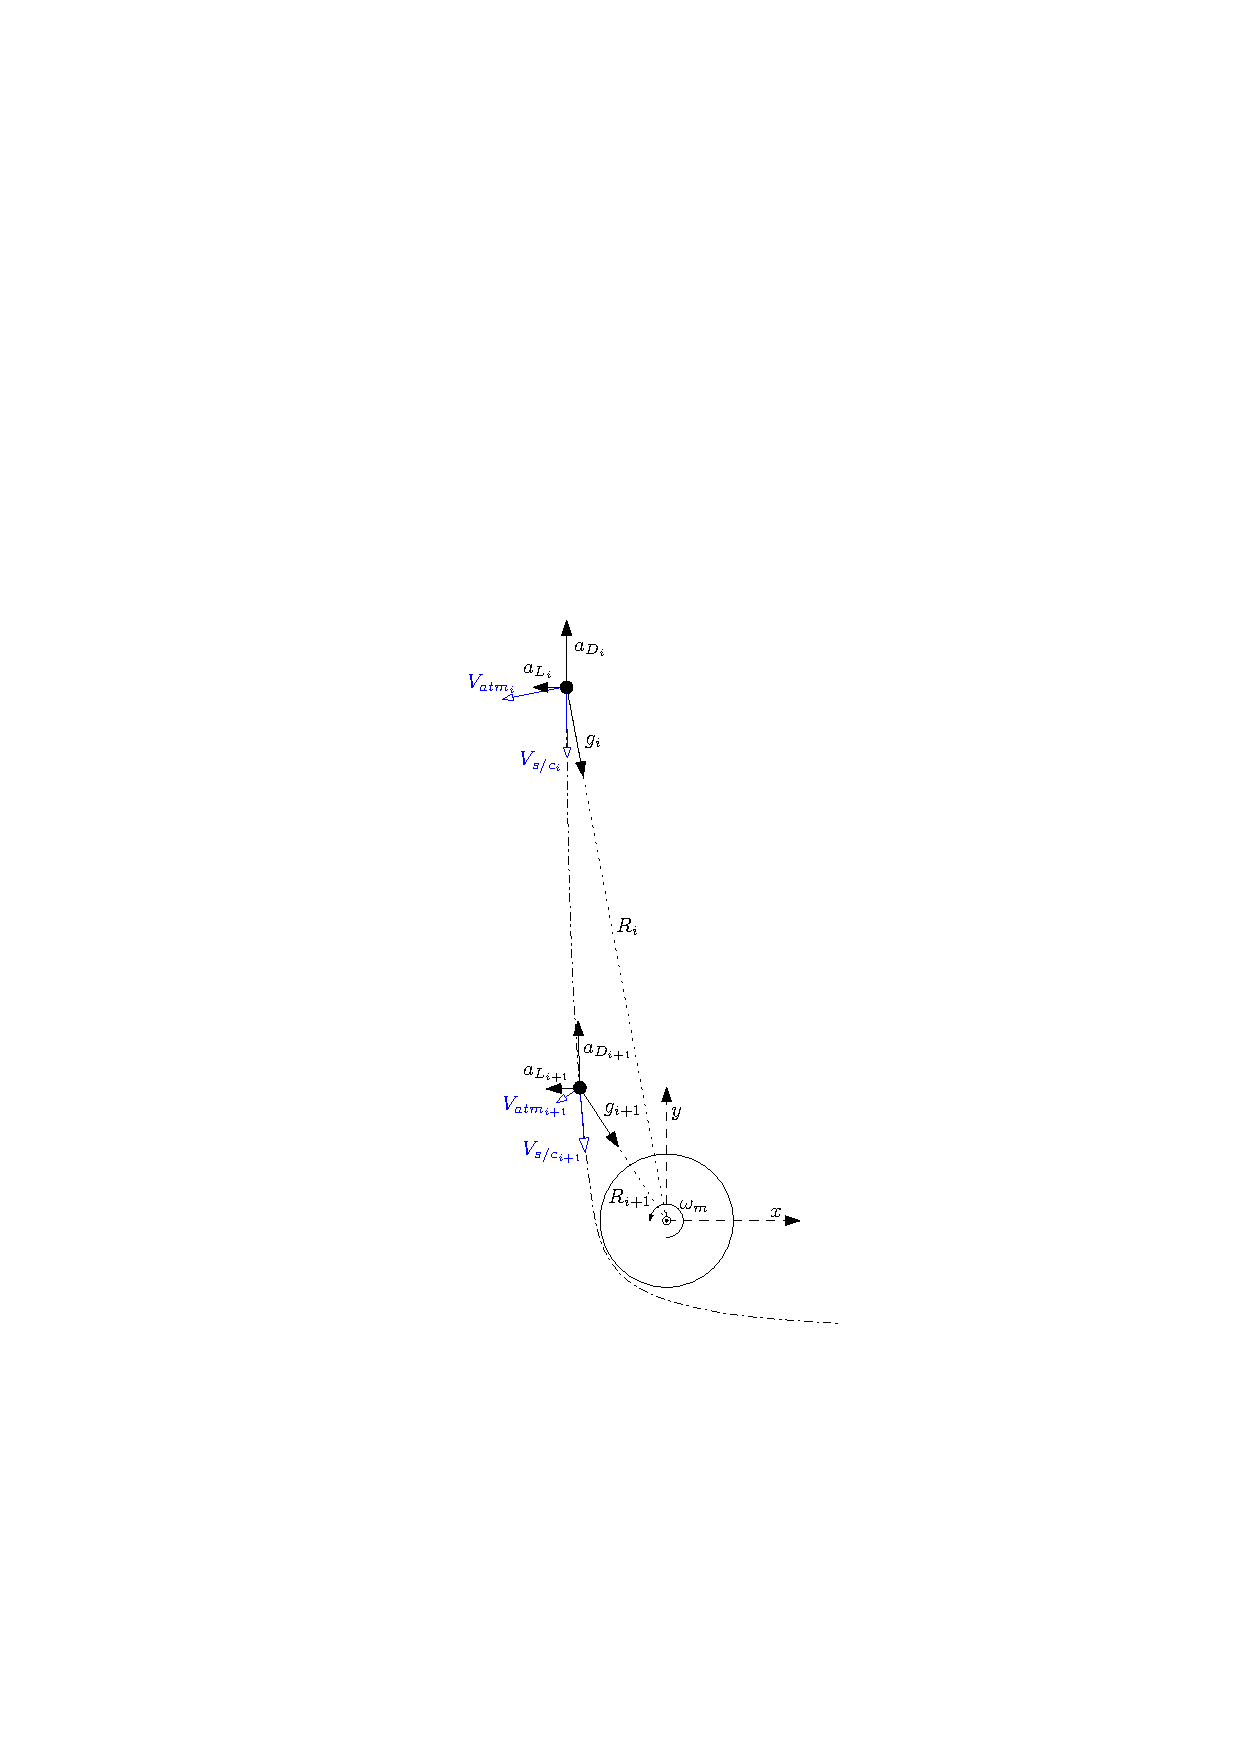
\includegraphics[width = 0.4\textwidth]{Figure/orbital_mechanics.pdf}
		\caption{The kinetic diagram visualizing the governing equations of the trajectory analysis}
		\label{fig:orb}
\end{wrapfigure}

The motion of a spacecraft can be broken down in some dominant contributors. These are the gravitational pull and the aerodynamic forces. Because the aerodynamic forces do have to be taken into account no Kepler orbit can be used.

To be able to fully describe the contributors, two reference frames need to be defined. The non-rotating inertial frame is defined with its origin in the centre of mass of Mars (if it would be perfectly spherical), this is the \gls{mci}. 
Another reference frame is the \gls{mcmf}, in our first model the origin and the z-axis of both reference frames are equal (so no axis tilt is taken into account). The difference between the two is that the \gls{mcmf} is rotating around the z-axis with rotational velocity \gls{con:omegamars} compared to the \gls{mci}.

The gravitational pull is described by Newton's law of gravitation, together with Newton's second law, it can be written as an acceleration as in equation \ref{eq:grav}.

The aerodynamic forces are described by the lift and the drag, these forces are acting in the negative direction and orthogonal to the velocity of the spacecraft with respect to the atmosphere as shown in Figure \ref{fig:orb}, this is the velocity of the spacecraft in the \gls{mcmf}. This velocity needs to be converted to \gls{mci} to be able to express the aerodynamic forces in the \gls{mci}, as in equation \ref{eq:Vsc_mcmf_mci}.

\begin{equation} \label{eq:Vsc_mcmf_mci}
\left.\gls{sym:Vvsc}\right|_{MCMF}^{MCI} = \gls{sym:Vvsc}_{,a} = \left.\gls{sym:Vvsc}\right|_{MCI} - \left(\gls{con:Omegamars} \times \gls{sym:Rv} \right)
\end{equation}

The aerodynamic accelerations due to the lift and the drag are described by equations \ref{eq:aL} and \ref{eq:aD} respectively \cite{AndersonJr.2007}.

\begin{equation} \label{eq:aL}
\gls{sym:aL} = \frac{\gls{sym:CL}\gls{sym:rho}\gls{sym:A}}{2 \gls{sym:m}} 
				\left|\gls{sym:Vvsc}_{,a}\right|^2
				\frac{\gls{sym:Vvsc}_{,a} \times \mathbf{z}}
				{\left| \gls{sym:Vvsc}_{,a} \times \mathbf{z}\right|}
\end{equation}

\begin{equation} \label{eq:aD}
\gls{sym:aD} = \frac{\gls{sym:CD}\gls{sym:rho}\gls{sym:A}}{2 \gls{sym:m}}
				\left|\gls{sym:Vvsc}_{,a}\right|^2 \frac{\gls{sym:Vvsc}_{,a}}{\left|\gls{sym:Vvsc}_{,a}\right|}
\end{equation}

The total acceleration is now the summation of the gravitational, lift and drag acceleration as in equation \ref{eq:aD}.

\begin{equation} \label{eq:acc}
\gls{sym:acc} = \gls{sym:g} + \gls{sym:aL} + \gls{sym:aD}
\end{equation}

Numerically differentiating the acceleration gives the Jerk $\left(\gls{sym:jerk}\right)$ This is done in equation \ref{eq:jerk}. Then the new position and velocity can be determined by discretizing the dynamic equations of motion resulting in equations \ref{eq:ai}, \ref{eq:Vi} and \ref{eq:Ri}.

\begin{equation} \label{eq:ai}
\gls{sym:acc}_i = \gls{sym:g}_i + \gls{sym:aL}_i + \gls{sym:aD}_i
\end{equation}

\begin{equation} \label{eq:jerk}
\gls{sym:jerk}_{i+1} = \frac{\gls{sym:acc}_{i-2} - 4\gls{sym:acc}_{i-1}+3\gls{sym:acc}_i}{2\gls{sym:Dt}}
\end{equation}

\begin{equation} \label{eq:Vi}
\gls{sym:Vv}_{i+1} = \gls{sym:Vv}_i + \gls{sym:acc}_i \gls{sym:Dt} + \frac{1}{2}\gls{sym:jerk}_i \gls{sym:Dt}^2
\end{equation}

\begin{equation} \label{eq:Ri}
\gls{sym:Rv}_{i+1} = \gls{sym:Rv}_i + \gls{sym:Vv}_i \gls{sym:Dt} + \frac{1}{2}\gls{sym:acc}_i \gls{sym:Dt}^2 + \frac{1}{6}\gls{sym:jerk}_i \gls{sym:Dt}^3
\end{equation}

\subsubsection{Eliptical Kepler orbit}
 \label{sec:eliptickep}
For an eliptical orbit \gls{sym:a}, \gls{sym:e} and \gls{sym:phip} can be calculated in the same way as was done in section \ref{sec:hypkep}. The point of reentry into the atmosphere is the old location exactly mirrored in the line between the pericenter and the apocenter. Also the velocity $\left(\gls{sym:Vv}\right)$ and the acceleration $\left(\gls{sym:acc}\right)$  should be mirrored in that line. The velocity should than be rotated over 180 $\left[^\circ\right]$ to point in the correct direction. The magnitude of the location $\left(\gls{sym:R}\right)$, velocity $\left(\gls{sym:V}\right)$ and acceleration $\left(\gls{sym:acc}\right)$ are still the same due to the symmetry of kepler orbits.

For the eliptical orbit also the duration has to be calculated. As this time is part of the 10 days in which the spacecraft is required to decelerate. As keplers second law states: $\frac{dA}{dt}=\mbox{constant}$, the duration can be written as an area fraction of the period. This is done in equation \ref{eq:areatime}. Here $\gls{sym:P} = 2\pi\sqrt{\frac{\gls{sym:a}^3}{\gls{con:mu}}}$ and $\gls{sym:A}_{tot} = 2\pi \gls{sym:a} \sqrt{1-\gls{sym:e}^2}$.

\begin{equation}
t = \frac{\gls{sym:A}}{\gls{sym:A}_{tot}}\gls{sym:P}
\label{eq:areatime}
\end{equation}

\subsection{Working principles of the tool}
\label{sec:astrowp}
The tool is able to calculate the trajectory of the spacecraft and a range of important parameters at each moment in time. These parameters are among others: Acceleration $\left(\gls{sym:acc}\right)$, dynamic pressure $\left(\gls{sym:q}\right)$, speed $\left(\gls{sym:Vv}\right)$ and Mach number $\left(\gls{sym:M}\right)$. In order to calculate this the tool takes geometric and aerodynamic properties of the spacecraft and some initial conditions as input.

***Flowchart + very short explanation***\\

\subsection{Verification \& validation}
\label{sec:astrovv}

In order to be sure the results the tool produces are correct and can safely be used in further efforts to design the \gls{cia} verification and validation is needed. This section presents the methods used to verify and validate the results produced by the tool. First a sensitivity analysis is presented in section \ref{sec:astrosens} which focusses on the sensitivity of the program to the initial conditions. In section \ref{sec:astrodisc} the discretisation error is analysed in order to ensure the results are accurate enough for it to be usefull. The numerical solution is compared to the simple case of a kepler orbit in section \ref{sec:astroverf}

\subsubsection{Sensitivity analysis}
\label{sec:astrosens}

In the sensetivity analysis the effect of a small change in input variables on the output is analysed. This effect was as expected for all variables except for the initial location. For all other variables the effect of a small change in input gave a small change in output. For the initial location however the effect of a small change in input gives a change of output orders of magnitude larger than the change in input. This large change can be explained by the long duration during which the spacecraft is attracted by a slightly different gravitational force. This force constantly increases the difference between the locations. this results in a difference in the order of kilometers in entry location for a difference in the order of millimeters in input location. It can thus be concluded that the model cannot be used as it is in this form, however this is not an error in the model. The model is correct and shows that in the future a controlsystem should be implemented in the simulation during the initial approach to diminish the increase in difference of location. This is also what will have to happen in reality on the spacecraft.

The temporary solution that was chosen to solve this problem is to take an initial location far closer to the planet. This induces an error because the initial conditions are no longer valid. The main error induced by this is the initial velocity that changes significantly between the sphere of influence \gls{soi} and the new initial condition which is located at ten times the mars radius above mars. Both have a variable distance to the left of mars. This difference in velocity is diminished by calculating the change in velocity from \gls{soi} to $10\cdot\gls{con:rm}$ for an orbit that starts straight above mars and using that difference in all other calculations aswell.

\subsubsection{Discretisation error}
\label{sec:astrodisc}

Due to the use of a discrete timestep an error relative to the real solution is induced. By testing the tool with the same initial conditions using different time meshes the difference between the solutions can be analysed. When the smallest timestep is assumed to be exact the error of the larger timesteps can be expressed relative to that. This relative error is shown in Figure \ref{fig:atmos_disc}. Please also note these errors are calculated running the tool without control.

Two conclusions can be drawn from this. First the error decreases quadraticaly with decreasing timestep. This means that the system converges to a solution. Secondly the error is smaller than 1 $\left[m\right]$ for a dt of smaller than $0.3 \left[s\right]$. This error is negligable compared to the error that will be induced by the assumptions that were made in section \ref{sec:astroassumption}.

%Initial Position
%rx = -4143775;
%ry = 10*R_m;
%R = [rx,ry,0];

%Initial Velocity
%v = 7.1679e+03; %[m/s]
%V = [0,-v,0];

\begin{figure}[h]
	\centering
	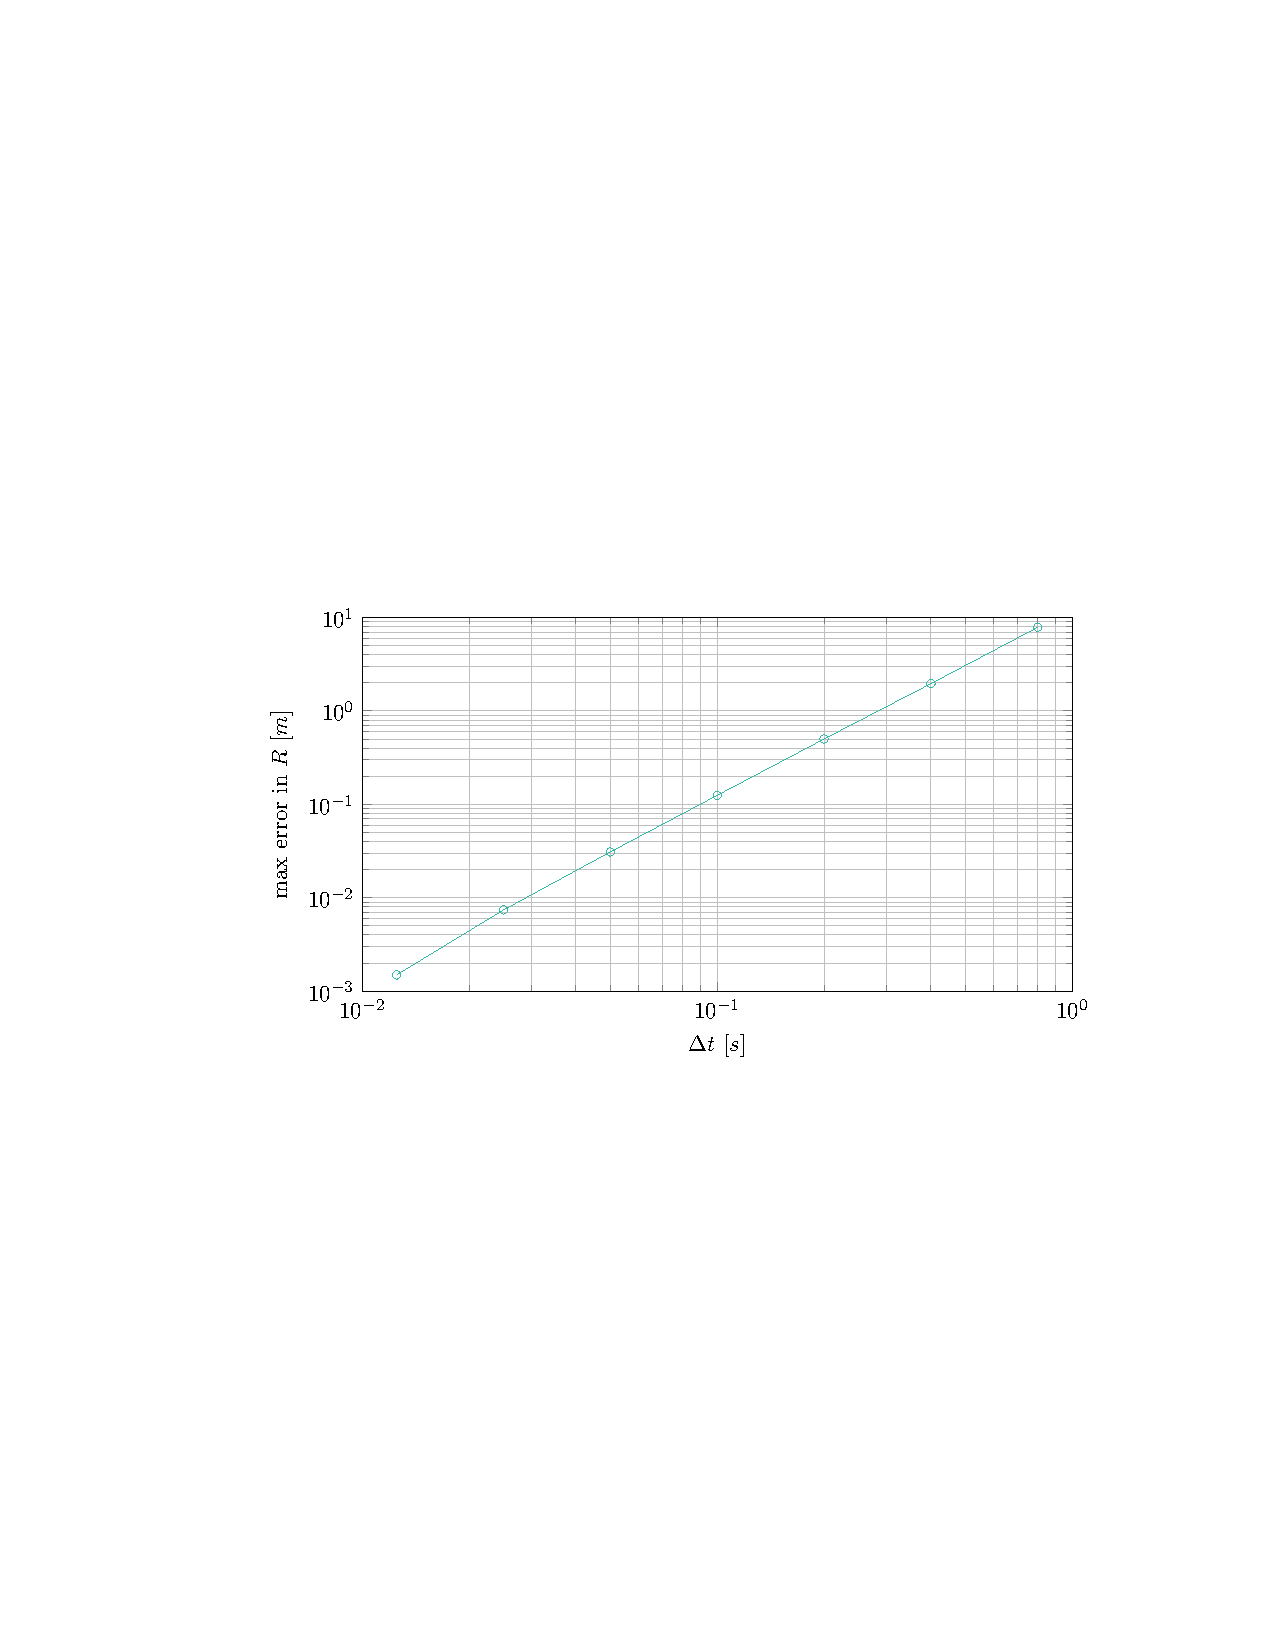
\includegraphics[trim={4.25cm 10cm 3.2cm 10cm},clip,width=0.8\textwidth]{Figure/orbital_model/dicretization.pdf}
	\caption{Discretisation error in radius $\left(\gls{sym:R}\right)$ after one pass through the atmosphere for initial position $\left[-4143775,10\cdot\gls{con:rm}\right]$ $\left[m\right]$ and initial velocity $\left[0,-7167.9\right]$ $\left[\frac{m}{s}\right]$ at $\gls{sym:alpha}=-10\left[^\circ\right]$ for the apollo shape}
	\label{fig:atmos_disc}
\end{figure}

\subsubsection{Verification through comparison with kepler}
\label{sec:astroverf}

In this section the results from the numerical simulation, which is usually only used in atmosphere, is compared to a kepler orbit. For this comparison the density is assumed to be zero, or in other words, it is assumed that there is no atmosphere. This comparison is done for different values of \gls{sym:Dt}. The error for each \gls{sym:Dt} is shown in Fig. \ref{fig:kep_error}.

%\begin{figure}[h]
%	\centering
%	\includegraphics[trim={4.25cm 10cm 3.2cm 10cm},clip,width=0.8\textwidth]{Figure/orbital_model/keplererror.pdf}
%	\caption{Error compared to a kepler orbit after 50005 seconds for initial position $\left[-4143775,10\cdot\gls{con:rm}\right]$ $\left[m\right]$ and initial velocity $\left[0,-7167.9\right]$ $\left[\frac{m}{s}\right]$ at $\gls{sym:alpha}=-10\left[^\circ\right]$ for the apollo shape}
%	\label{fig:kep_error}
%\end{figure}

The figure shows the error is between 15 and 5 for \gls{sym:Dt} between 1 and 0.01. The error decreases, but seems to tend to a non-zero constant value. The method used for numeical simulation is thus convergent, but has a small offset from the exact solution. This error is however so small it can easily be accepted.

%\subsection{Performance of control systems}
% \label{sec:astroref}
%Several options for the control system are considered. Using first-order calculations the effectiveness of each control system design option will be assessed. In this context 'effectiveness' is defined as a combination of system mass, moment that can be caused by the system and whether a control output can be sustained for long periods of time. These three criteria will be considered for all three control system design options. The design options to be considered are:
%\begin{itemize}
%	\item Shifting the \acrfull{cg}
%	\item A \acrfull{rcs}
%	\item Control surfaces (body flaps)
%\end{itemize}
%Each of these options will be quickly assessed in the subsequent sections. This will be done by taking angle of attack \gls{sym:alpha}$=30\deg$. This corresponds to $\gls{sym:CM}\gls{sym:A}=-100$, $\gls{sym:CL}\gls{sym:A}=-58.8$ and $\gls{sym:CD}\gls{sym:A}=126$. These values have been obtained by using the aerodynamical tool described in chapter \ref{ch:aero_analysis} for an Apollo-shaped object. Using equation \ref{eq:moment_from_cm} the control moment required can be obtained.
%\begin{equation}
%M=\frac{1}{2}\gls{sym:rho}\gls{sym:V}^{2}\gls{sym:CM}\gls{sym:A}
%\label{eq:moment_from_cm}
%\end{equation}
%This moment has to be counteracted during a time $t$. Furthermore, for the \gls{rcs} and body flaps the required force can be directly determined by noting that $M=dF$, where $d$ is the moment arm and $F$ is the control force. 
%
%\subsubsection{\gls{cg}-shifting}
%By moving the \acrlong{cg} of the spacecraft the sum of the moments exerted on it changes. This will cause a change in spacecraft attitude, thereby also trimming the capsule. The \gls{cg}-shift can be achieved by shifting the location of the aeroshell with respect to the capsule. This will slightly move the \acrlong{cg} of the spacecraft and change the location of the lift and drag forces acting on it. In order to avoid over-designing the actuator concerned with shifting the aeroshell with respect to the capsule (and thus making it heavier) the movement speeds are limited to low values.
%
%\subsubsection{\acrlong{rcs}}
%By using the control force requirement the mass flow of the \acrlong{rcs} can be determined with equation \ref{eq:rcsmassflow} \cite{Allen2012}.
%\begin{equation}
%\frac{M}{d}=F=\gls{sym:mdot}\gls{sym:Isp}\gls{sym:ge}
%\label{eq:rcsmassflow}
%\end{equation}
%From equation \ref{eq:rcsmassflow} the required propulsive mass can be obtained by multiplying both sides of the equation with timespan $t$ and solving for $\gls{sym:m}$, which results in equation \ref{eq:propmass}.
%\begin{equation}
%\gls{sym:m}=\frac{Ft}{\gls{sym:Isp}\gls{sym:ge}}
%\label{eq:propmass}
%\end{equation}
%
%By working out equation \ref{eq:propmass} one can see that the required propulsive mass $\gls{sym:m}=$. From this it can be observed that using a control system relying exclusively on rocket control is not reconcilable with the weight requirements imposed on the hypersonic decelerator.
%\subsubsection{Body flaps}
%Body flaps function by introducing a local aerodynamical force by controlling the local geometry. A body flap element produces a lift and drag force as in equation \ref{eq:flaplift} and \ref{eq:flapdrag}.
%\begin{multicols}{2}
%\begin{equation}
%L=\frac{1}{2}\gls{sym:rho}\gls{sym:V}^{2}\gls{sym:CL}\gls{sym:A}
%\label{eq:flaplift}
%\end{equation} \break
%\begin{equation}
%D=\frac{1}{2}\gls{sym:rho}\gls{sym:V}^{2}\gls{sym:CD}\gls{sym:A}
%\label{eq:flapdrag}
%\end{equation}
%\end{multicols}
%Consider figure \ref{fig:flapstuff}. It can be seen that the moment around the \gls{cg} caused by an drag of an element at a distance is equal to 
%\begin{figure}
%	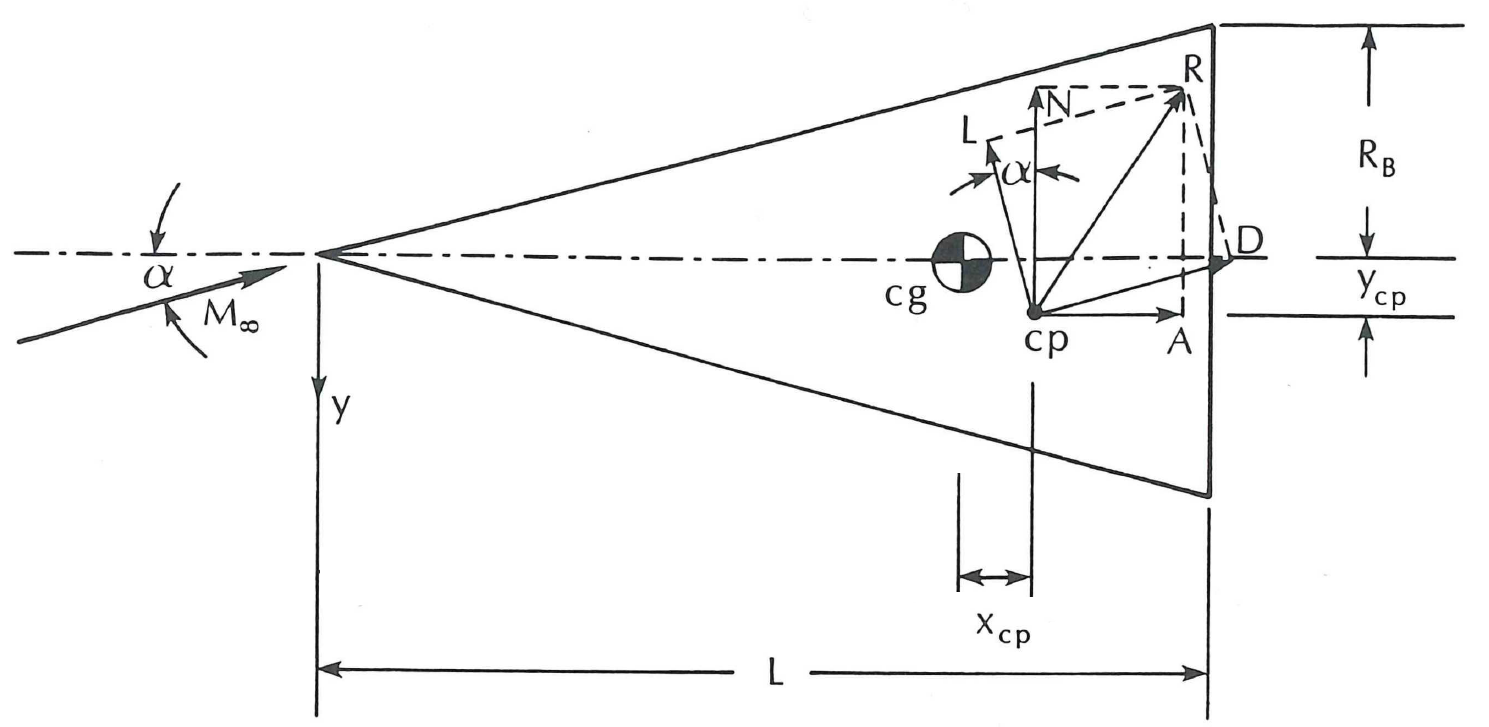
\includegraphics[width=0.7\textwidth]{./Figure/def_flap_distances}
%	\caption{Definition of flap moment arms}
%	\label{fig:flapstuff}
%\end{figure}
%By noting that both of these forces cause a moment
%\subsubsection{Control system design conclusions}
%From the previous sections one can conclude that all proposed concepts have their own strengths and weaknesses. In order to combine these it has been decided to combine \gls{cg}-shifting with
%
%
%***Moment or dalpha/dt that control systems (cg offset, thrusters, control surfaces) can create***\\
%***Weight estimate of each control system (per concept if needed)***\\

\subsection{Results \& conclusions}
\label{sec:astrores}
In this section the results from the astrodynamics \& control are presented. Furthermore the required performance of the controlsystem is analysed and a conclusion is drawn on which control systems are feasible.

In section \ref{sec:astroatmos} the data from the atmospheric model is shown. This data is used as a primary input for the computations. Section \ref{sec:astrodec} shows the effect of angle of attack $\left(\gls{sym:alpha}\right)$ on the maximum deceleration during a trajectory for which the spacecraft goes into orbit. In section \ref{sec:astroperfomance} the required performance of the control system is analysed. In section \ref{sec:astrorestraj} one of the trajectories which was found to be feasible in section \ref{sec:astroperfomance} is shown and the important parameters, most of which will serve as input for other tools, are analysed. In section \ref{sec:conclusion} a conclusion is drawn about which control system can meet the required controler performance.

\subsubsection{Atmospheric model}
\label{sec:astroatmos}

In this section the data from the atmospheric model is presented. This data is of upmost importance for our tool to work properly.

The data that is most important to us is the variation of density $\left(\gls{sym:rho}\right)$ and temperature $\left(\gls{sym:T}\right)$ with height. these relations are shown in figure \ref{fig:atmos_height}.

\begin{figure}[ht!]
	\centering
	\begin{subfigure}{0.45\textwidth}
	\centering
	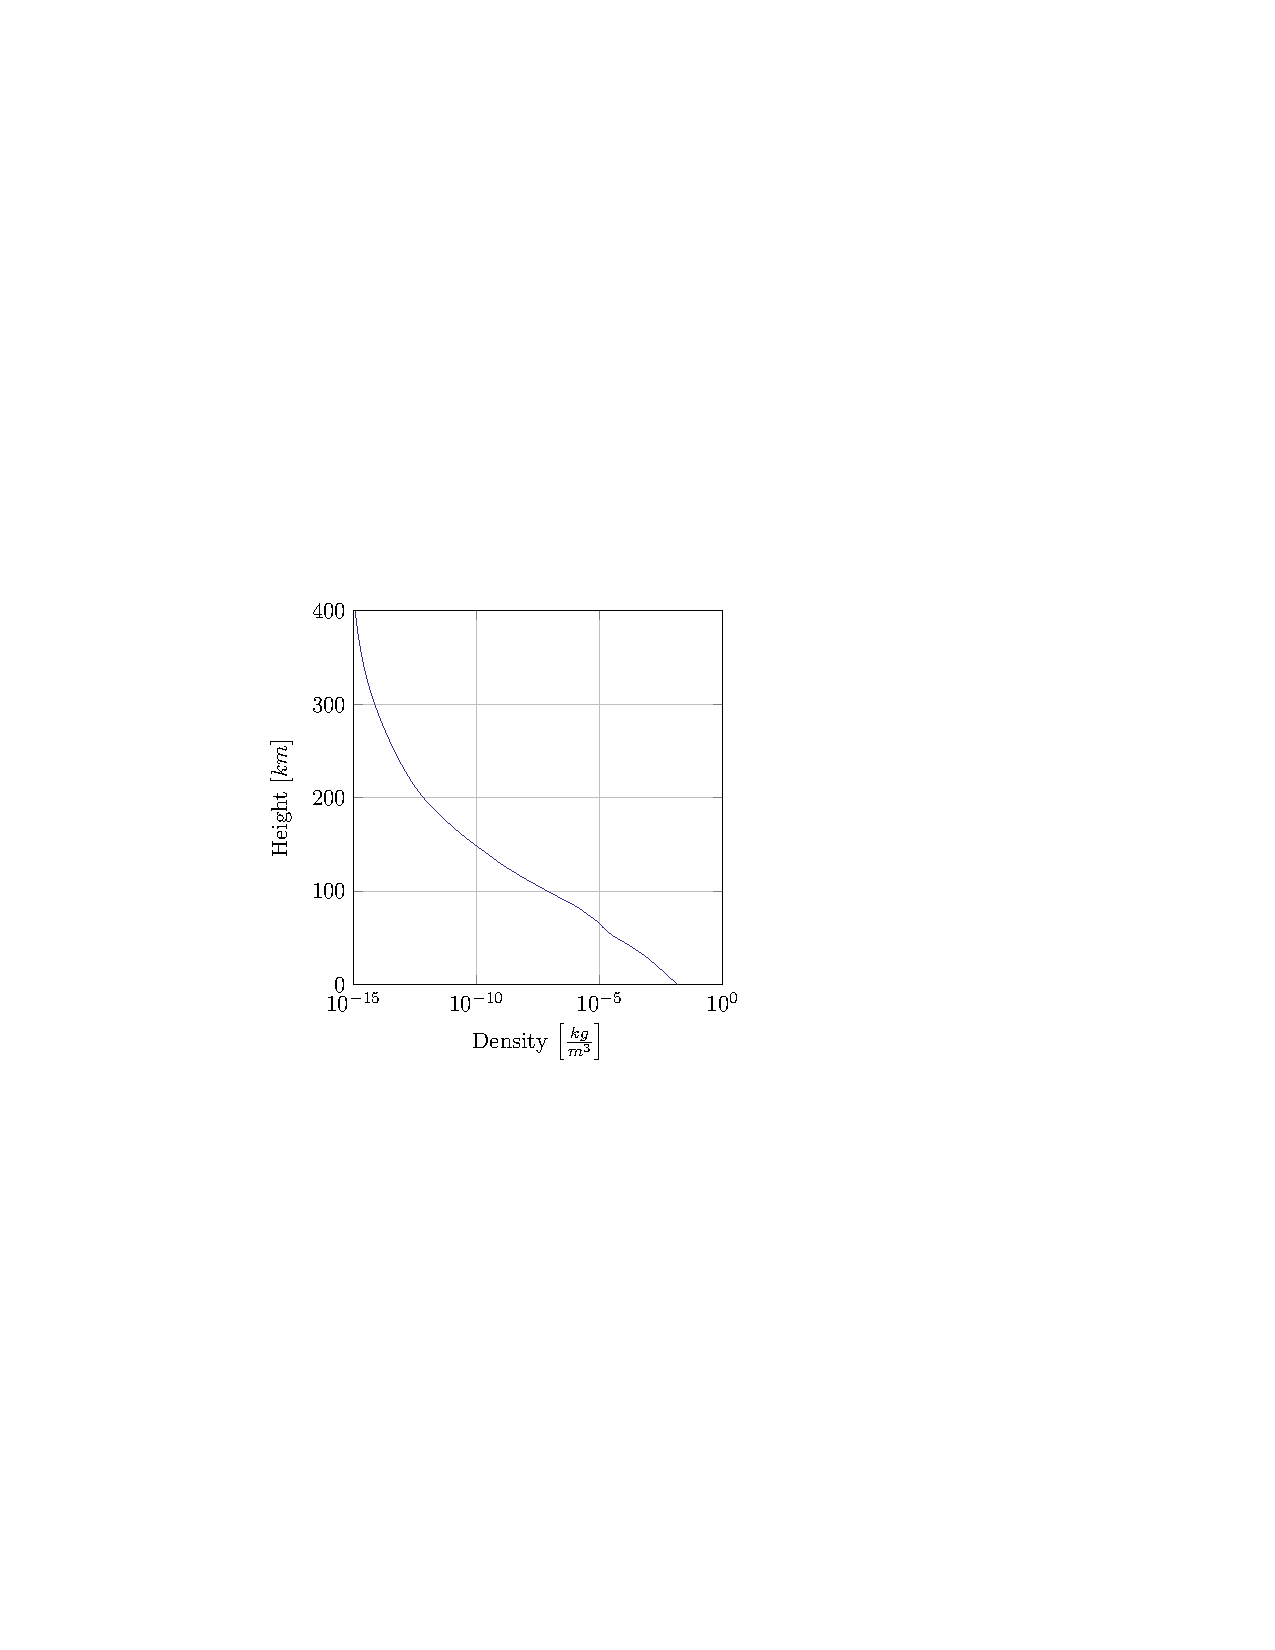
\includegraphics[trim={4cm 9.8cm 9cm 10cm},clip,width=0.9\textwidth]{Figure/atmos_model/density.pdf}
	\caption{The atmospheric density} 
	\label{fig:atmos_height_rho}
	\end{subfigure}
	\begin{subfigure}{0.45\textwidth}
	\centering
	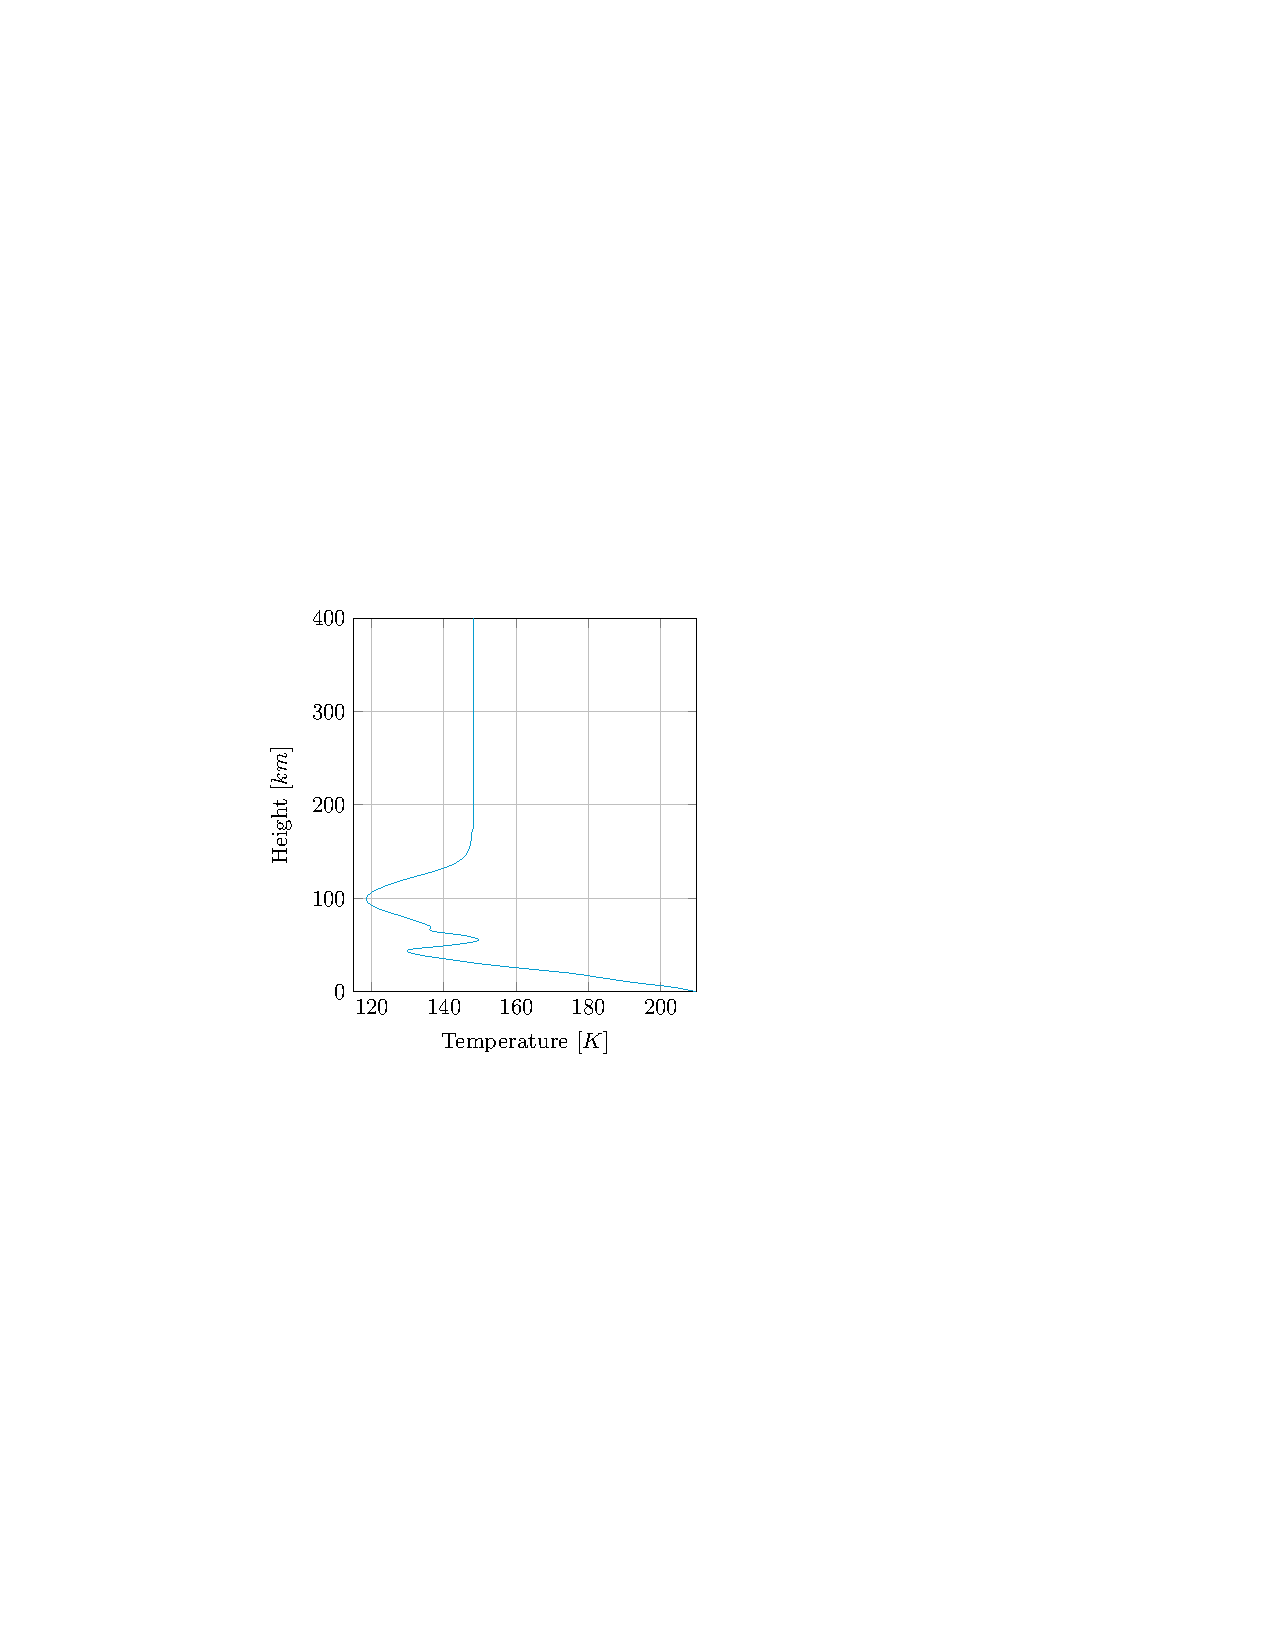
\includegraphics[trim={4cm 9.8cm 9cm 10cm},clip,width=0.9\textwidth]{Figure/atmos_model/temperature.pdf}
	\caption{The atmospheric temperature}
	\label{fig:atmos_height_T}
	\end{subfigure}
	\caption{The atmospheric properties for different heights}
	\label{fig:atmos_height}
\end{figure}

As was already stated in section \ref{sec:astroassumption} the atmospheric properties are assumed to be equal over different longitudes. That this is not exacly true can be seen in figure \ref{fig:atmos_lon}. In order for this assumption to induce as little error as possible a constant longitude at which all atmospheric properties are approximately at their average has been chosen to do the calculations with. The longitude that fits this description best for different heights is $180 \left[^\circ\right]$.

\begin{figure}[ht!]
	\centering
	\begin{subfigure}{0.9\textwidth}
	\centering
	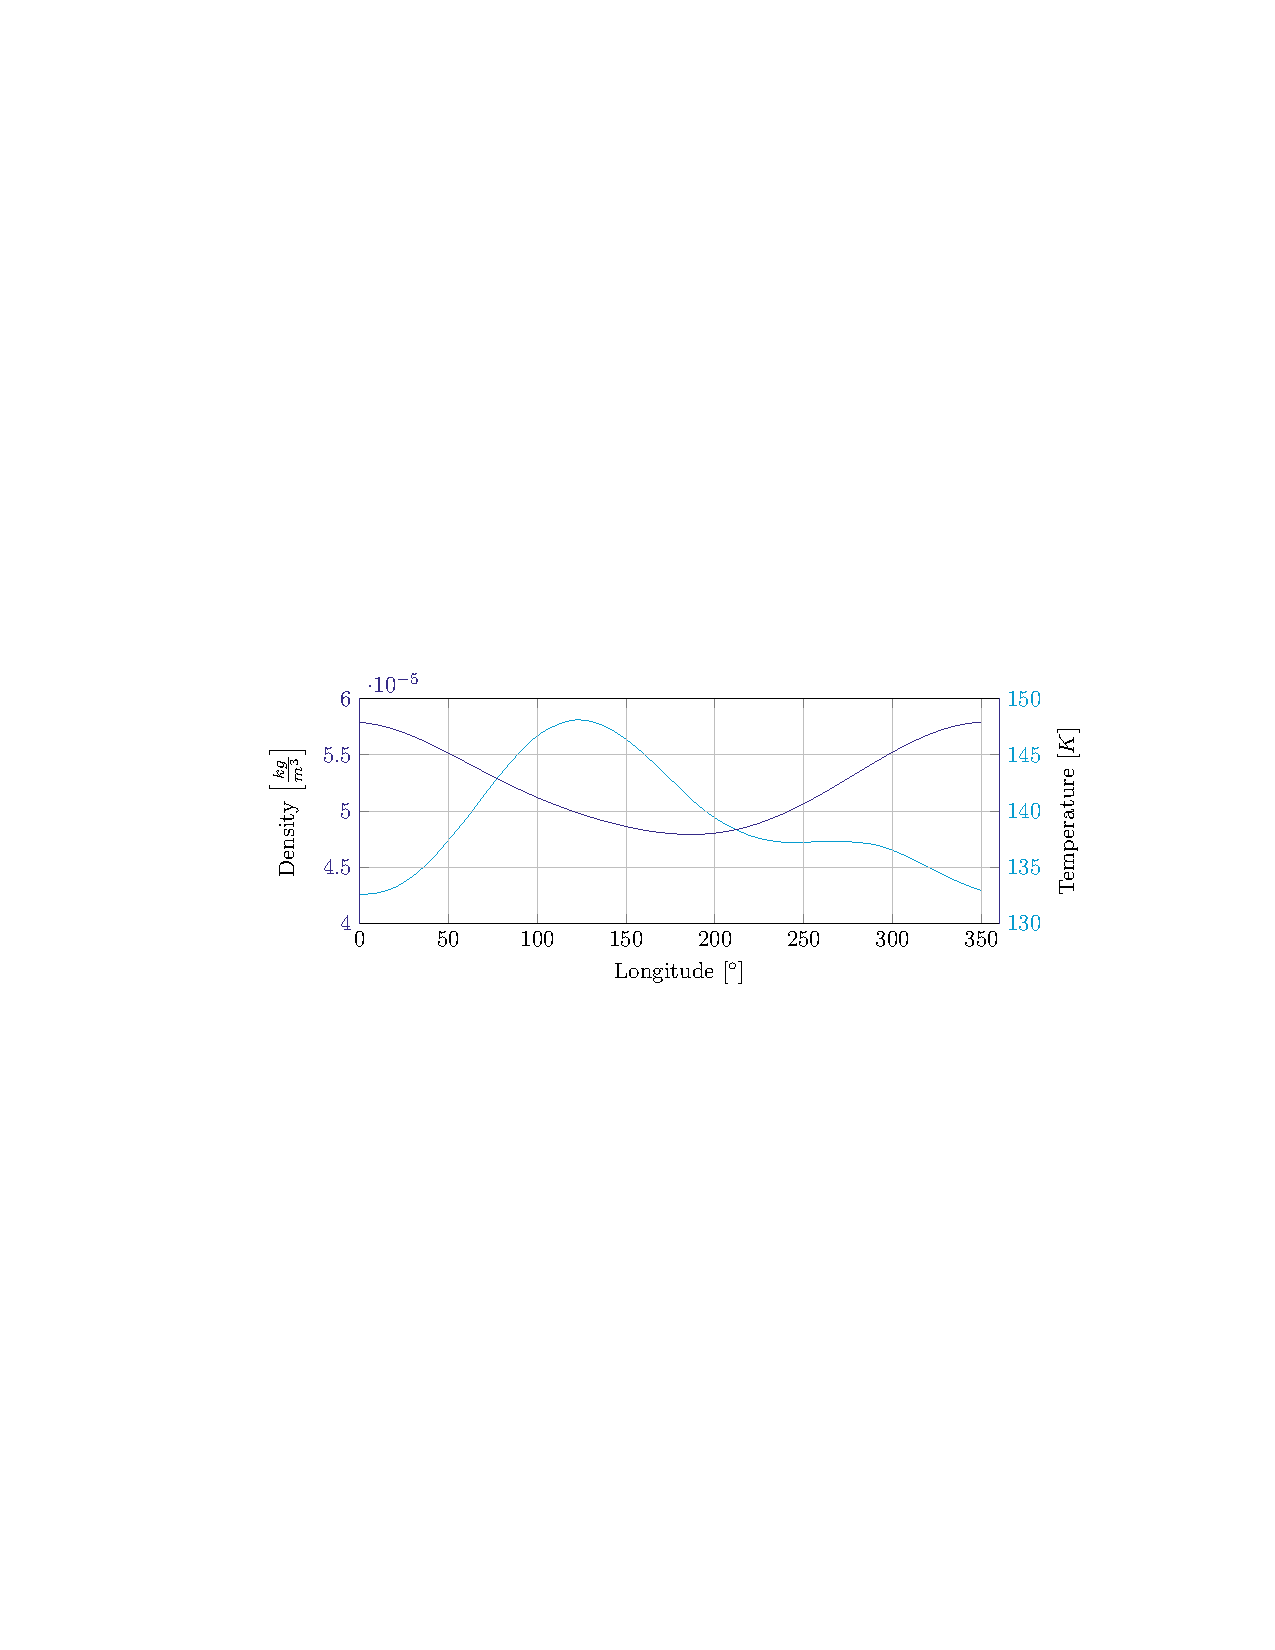
\includegraphics[trim={4.25cm 11cm 3.2cm 11cm},clip,width=0.9\textwidth]{Figure/atmos_model/lon_50.pdf}
	\caption{The atmospheric properties at $50$ $\left[km\right]$} 
	\label{fig:atmos_lon_50}
	\end{subfigure}
	\begin{subfigure}{0.9\textwidth}
	\centering
	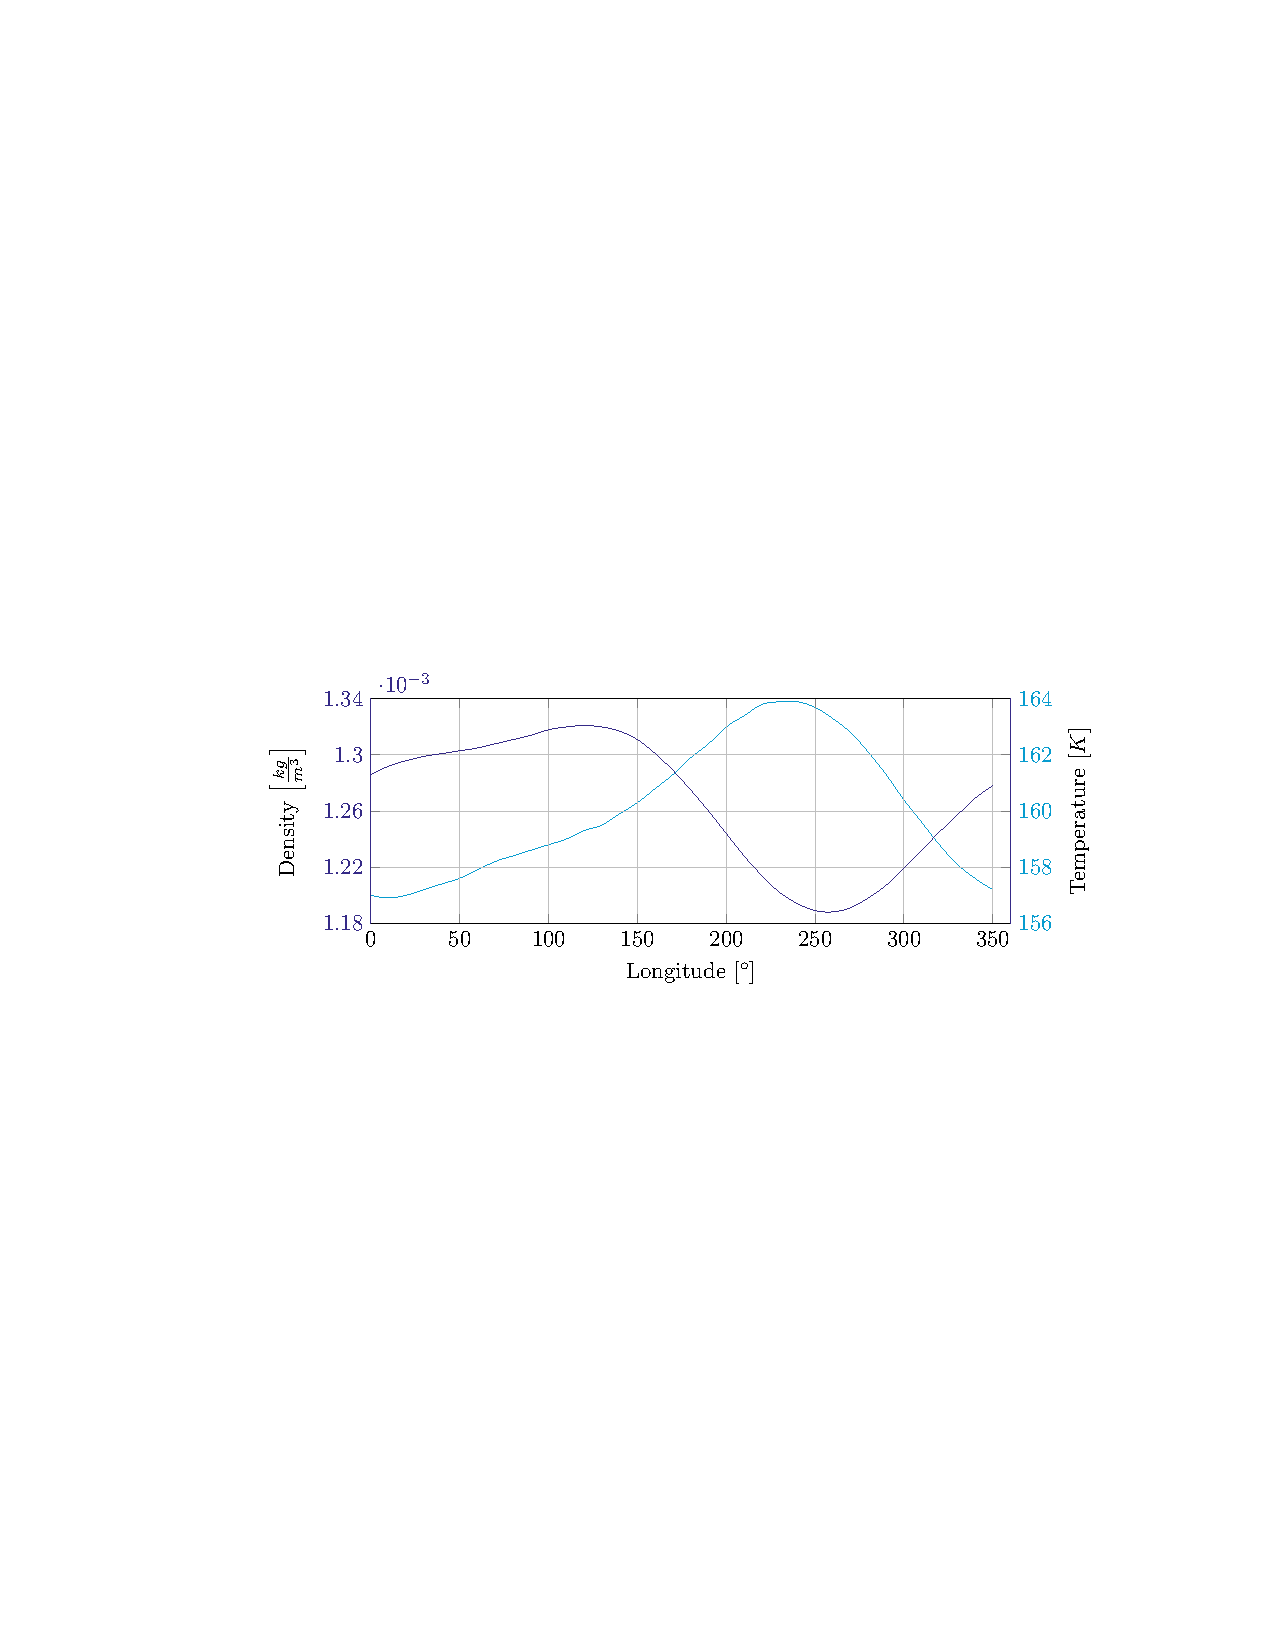
\includegraphics[trim={4.5cm 11cm 3.1cm 11cm},clip,width=0.9\textwidth]{Figure/atmos_model/lon_25.pdf}
	\caption{The atmospheric properties at $25$ $\left[km\right]$} 
	\label{fig:atmos_lon_25}
	\end{subfigure}
	\caption{The atmospheric properties for different heights at a latitude of 0 $\left[^\circ\right]$}
	\label{fig:atmos_lon}
\end{figure}

\subsubsection{Effect of \gls{sym:alpha} on deceleration}
\label{sec:astrodec}

In this section the effect of the angle of attack $\left(\gls{sym:alpha}\right)$ on the maximum load endured during an orbit is discussed. In figure \ref{fig:n_alpha} this effect is shown for all of the different concepts. The figure for stacked toroid is the same as the figure for the tension cone. All combinations of \gls{sym:alpha} and $\gls{sym:acc}_{max}$ in the coloured part of the graphs are feasible orbits. For all combinations above the coloured part the spacecraft crashes. For all combinations underneath the coloured part the spacecraft flies past Mars without getting into orbit. It is clear from these graphs that there is no concept for which an orbit can be found with a maximum acceleration of less than the required $3 \gls{sym:g} \left[\frac{m}{s^2}\right]$. From this it can be concluded that the spacecraft needs active control to find an orbit which meets the requirements.

\begin{figure}[h]
	\centering
	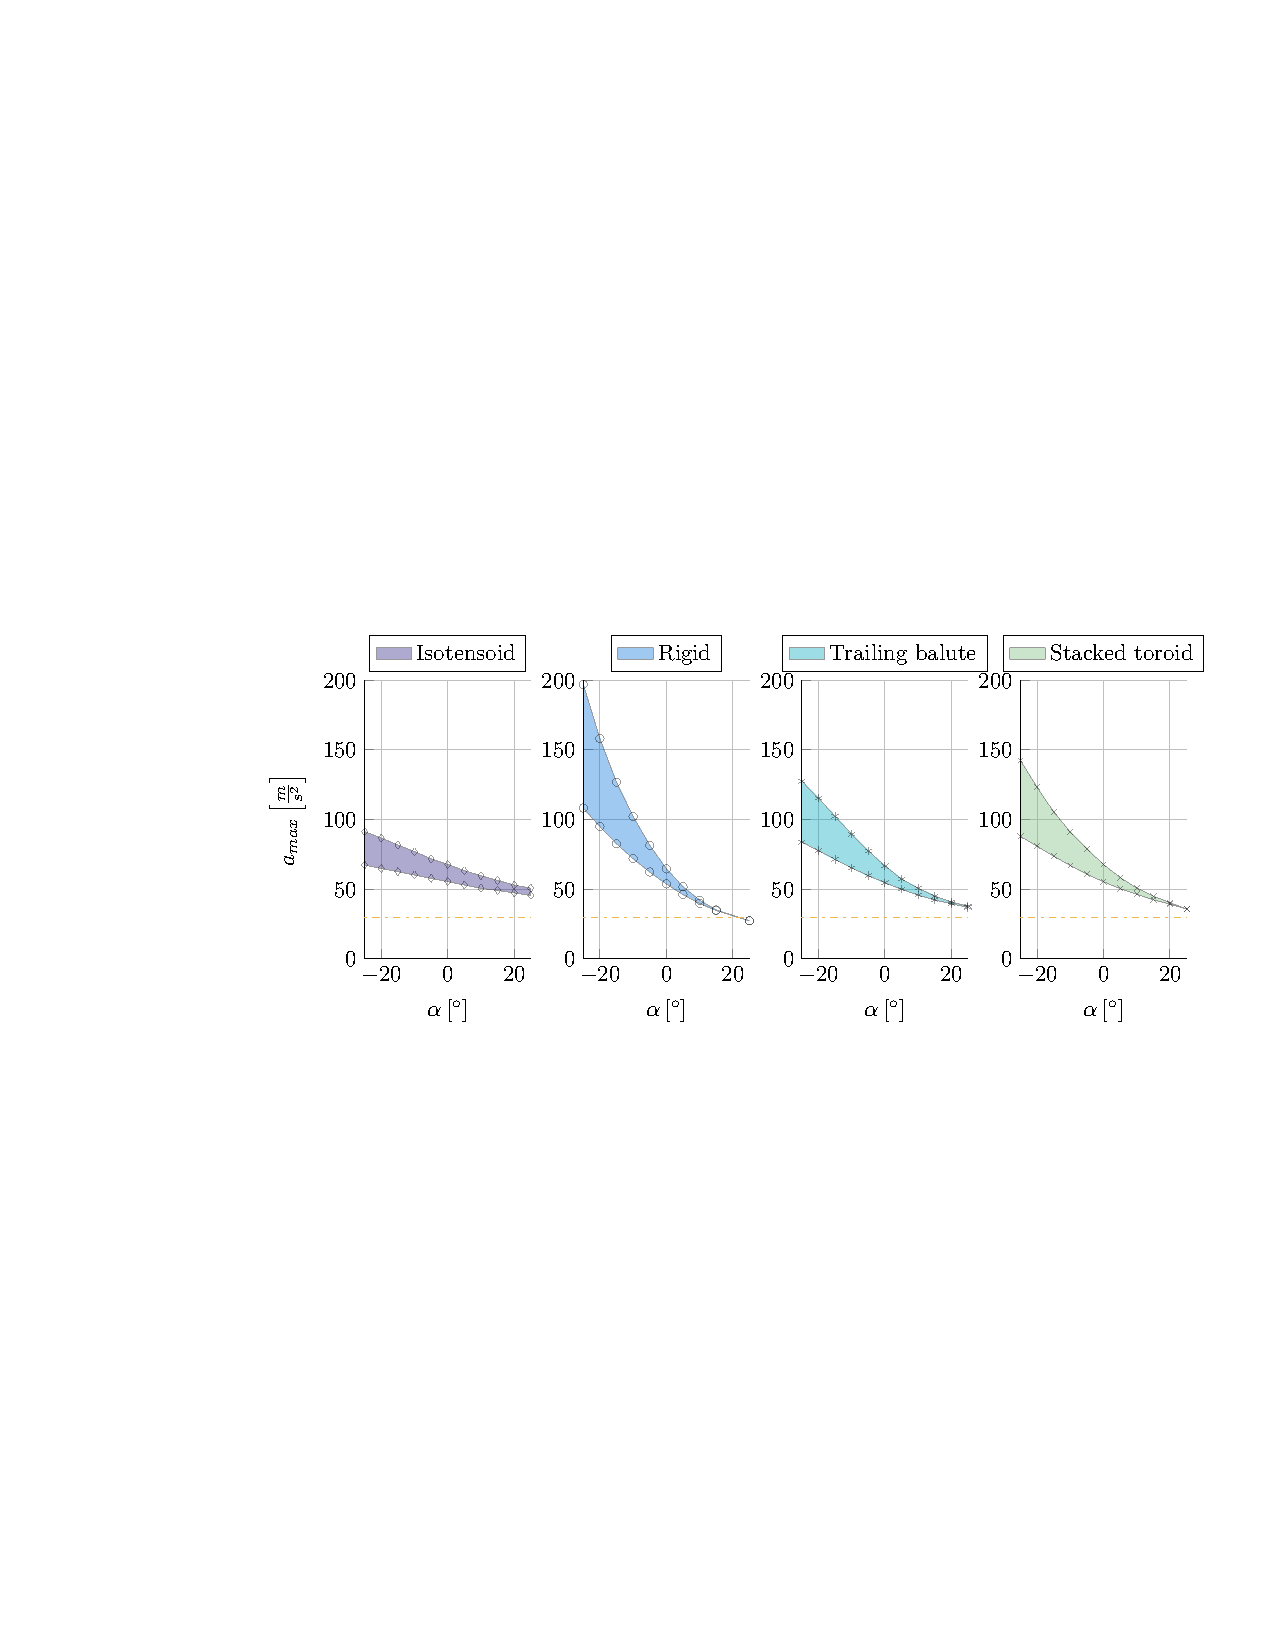
\includegraphics[trim={4.25cm 10.5cm 1cm 10.5cm},clip,width=0.95\textwidth]{Figure/orbital_model/n_alpha.pdf}
	\caption{Possible trajectories for which the spacecraft goes into orbit without control.}
	\label{fig:n_alpha}
\end{figure}

\subsubsection{Required performance of the control system}
\label{sec:astroperfomance}

In section \ref{sec:astrodec} it was found that a control system will be needed to find an orbit that meets the requirements. In this section the required performance of the control system is outlined and some important parameters with respect to this performance are explained.

The control system is required to force the acceleration into a rectangular shape as much as possible. This rectangle should have a height of $3 \gls{sym:g} \left[\frac{m}{s^2}\right]$ acceleration and a width of the time the spacecraft is in the atmosphere. This shape is not even achievable with infinitely good control as the atmosphere is too thin at the outer edges. However with rounded off edges this shape is very well possible. Whether the initial rise has an overshoot, how well the upper limit can be kept and how far the sides of the rectangle are separated is dependent on the performance of the control system.

***Results of needed CLmax, dalpha/dt, dCL/dalpha***\\

\subsubsection{A feasible trajectory and important output parameters over time}
\label{sec:astrorestraj}

In this section a controlled orbit for each concept is shown. This is done to show which values for i.e. dynamic pressure $\left(\gls{sym:q}\right)$ are reasonable to use in the other tools.

\paragraph{Stacked toroid/tension cone}

\paragraph{Rigid}

\paragraph{Isotensoid}

\paragraph{Trailing Ballute}

***Plot of a trajectory***\\
***Plots of output variables for that particular trajectory***\\

\subsubsection{Conclusion on control system performance}
\label{sec:conclusion}
As stated in section \ref{
